\section{GPU Parallelisierung}
\textbf{GPU:} Extrem hohe Datenparallelität, Wenig Verzweigungen, Kein beliebiges Warten bei Parallelität, Einfache aber viele Cores, Kleine Caches pro Core \\
\textbf{CPU:} Niedrige Datenparallelität, Viel Verzweigungen, Beliebige Thread-Synchronisation, Wenige aber mächtige Cores, Grössere Caches per Chip

\textbf{Arithmetic Intensity:} (FLOP per Byte ratio) Je höher desto besser auf parallelen Prozessoren. 
\[ ArithmeticIntensity = \frac{BWcompute}{BWmemory} \]

\subsection{GPU Aufbau (Physikalisch)}
\begin{minipage}[t]{0.33\linewidth}
	\textbf{Shared Memory} \\
	Pro Streaming Multiprozessor \\
	Zugriff: \lstinline|__shared__ float x;| \\
	Schnell, ca 4 Zyklen \\
	Paar KiloBytes
\end{minipage}
\begin{minipage}[t]{0.33\linewidth}
	\textbf{Global Memory}\\
	Main Memory \\
	Zugriff \lstinline|cudaMalloc()|
	Langsam, ca. 400-600 Zyklen pro Zugriff \\
	in Allen Threads sichtbar \\
	Mehrere GB
\end{minipage}
\begin{minipage}[t]{0.33\linewidth}
	\textbf{Local Memory} \\
	Per Thread (Spill over) \\
	Befindet sich im Global Memory \\
	Nur für den Thread sichtbar
\end{minipage}

\textbf{SIMD (Vektor-Parallelität:} Alle Threads führen denselben Kernel-Code aus. Die Ausführung unterscheidet sich nur in den Werten von threadIdx und blockIdx. Zu einem Zeitpunkt führen alle Threads (konkret in einem Warp) dieselbe Instruktion auf (typischerweise) verschiedenen Daten aus. Bei Verzweigungen werden die Instruktionen der Pfade abwechselnd ausgeführt. Threads ignorieren dabei die Instruktionen eines anderen Pfades.

\textbf{Divergenz:} gibt es Threads innerhalb eines Warps, die unterschiedliche Dinge tun? (logische if, else Verzweigung) -> schlecht, alle anderen Threats warten in dieser Zeit.

\textbf{Memory Coalescing:} Es sollte immer in 32 Byte (= 4 ints) Blöcken (oder vielfachen) in 32Byte Abständen auf den Speicher zugegriffen werden, sonst braucht es mehrere Memory Zyklen.  

\textbf{CUDA Barriere} \lstinline|__syncthreads();|  // synchronisiert alle Threads innerhalb eines Blocks, damit alle Threads gleichzeitig durch diesen Punkt gehen. Achtung: Falls in if/else Block, sind if oder else case zwei unterschiedliche Barrieren!

\subsection{Beispiele}
\textbf{Einfacher Kernel zu Vektor-Addition}
\begin{lstlisting}[style=csharp]
__global__
void vecAKern(float *A, float *B, float *C, int N) {
	int i = blockIdx.x * blockDim.x + threadId.x;
	if (i < N) { C[i] = A[i] + B[i]; }
	// alle anderen Threads machen nichts
}
\end{lstlisting}  

\textbf{Kernel für die Vektor-Addition}
\begin{lstlisting}[style=csharp]
#include <stdio.h>
#include <cuda.h>

#define N 10000

__global__ 
void add(int *a, int *b, int *c)
{
    int tid = blockDim.x * blockIdx.x + threadIdx.x;
    if (tid < N) {
        c[tid] = a[tid] + b[tid];
    }
}
int main() {
    int *a, *b, *c;
    int *d_a, *d_b, *d_c;

    a = (int*) malloc( N * sizeof(int) );
    b = (int*) malloc( N * sizeof(int) );
    c = (int*) malloc( N * sizeof(int) );

    cudaMalloc( &d_a, sizeof(int) * N);
    cudaMalloc( &d_b, sizeof(int) * N);
    cudaMalloc( &d_c, sizeof(int) * N);

    cudaMemcpy( d_a, a, N * sizeof(int), cudaMemcpyHostToDevice);
    cudaMemcpy( d_b, b, N * sizeof(int), cudaMemcpyHostToDevice);

    int blockSize = 1024;
    int gridSize = (N + numThread - 1) / numThread;

    add<<<gridSize, blockSize>>>( d_a, d_b, d_c );
    cudaDeviceSynchronize();

    cudaMemcpy( c, d_c, N * sizeof(int), cudaMemcpyDeviceToHost);
   
    free( a ); free( b ); free( c );
    cudaFree( d_a ); cudaFree( d_b ); cudaFree( d_c );   
}
\end{lstlisting}

\subsection{Roof Line Model}
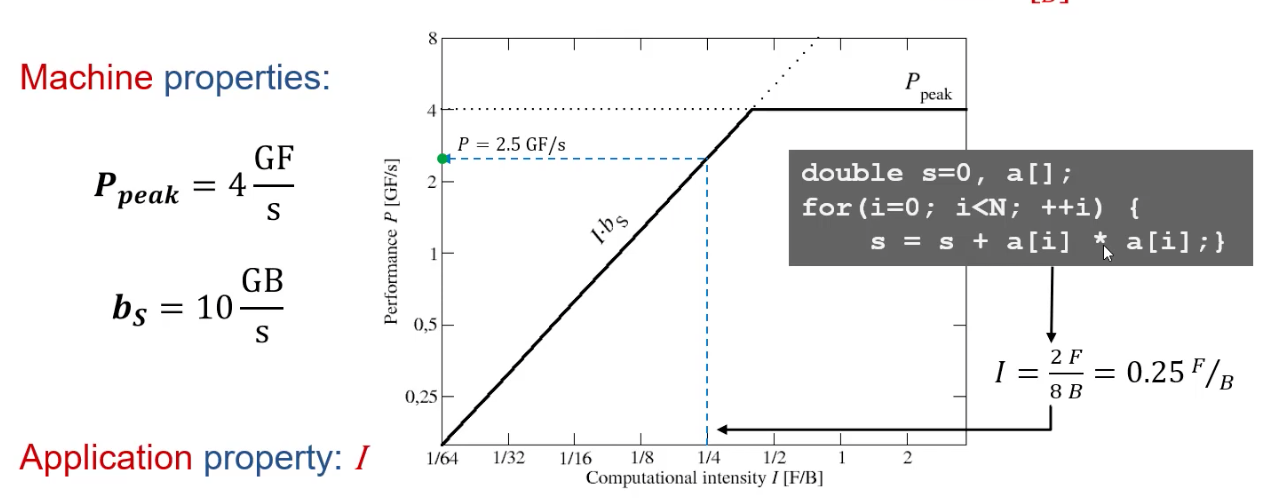
\includegraphics[width=\linewidth]{rooflinemodel.png}

\section{Cluster Programming}
\begin{description}
	\itemsep -0.2em
	\item [Shared Memory] (SMP, POSIX, OpenMP)
	\item [Distributed Memory] / Message Passing (MPI)
	\item [Single Program Multiple Data] (SPMD)
	\item [Multiple Program Multiple Data] (MPMD)
	\item [HPC Hybrid] Memory Model SPMP mit mehreren Nodes
\end{description}

\subsection{Message Passing Interface (MPI)}
\lstinline|MPI_Init(&argc, &argv);| Initialisierung von MPI \\
\lstinline|MPI_Comm_rank(MPI_COMM_WORLD, &rank);| identifiziert Prozessor in der Gruppe nach Rang \\
\lstinline|MPI_Comm_size(MPI_COMM_WORLD, &size);| Grösser der MPI Gruppe \\
\lstinline|MPI_Send(&value, length, type, receiverRank, tag, MPI_COMM_WORLD);| \\
\lstinline|MPI_Recv(&value, length, type, senderRank, tag, MPI_COMM_WORLD, MPI_STATUS_IGNORE);| \\
\lstinline|MPI_Finalize();| Aufräumen der Umgebung

\textbf{Datentypen:} MPI\_CHAR, MPI\_SHORT, MPI\_INT, MPI\_LONG, MPI\_LONG\_LONG, MPI\_UNSIGNED, MPI\_FLOAT, MPI\_DOUBLE

\textbf{Broadcast:} \lstinline|MPI_Bcast(&data, int length, type, receiverRank, MPI_COMM_WORLD);|

\textbf{MPI Barrier:} \lstinline|MPI_Barrier(MPI_COMM_WORLD);|

\textbf{Reduktion:} Operationen auf allen Teilen anwenden und zu einem Ergebnis kalkulieren

\begin{lstlisting}[style=csharp]
// Jeder Prozess erhaelt das Resultat
MPI_Allreduce(&localValue, &totalValue, length, type, aggregator, MPI_COMM_WORLD);	
// Nur ein Prozess erhaelt das Resultat
MPI_Reduce(&localValue, &totalValue, length, type, aggregator, receiverRank, MPI_COMM_WORLD); 
\end{lstlisting}

\textbf{Senden von Werten von einem Prozess an alle anderen (Broadcast)}
\begin{lstlisting}[style=csharp]
int main(int argc, char * argv[]) 
{
    int rank, size;
    
    MPI_Init(&argc, &argv);

    MPI_Comm_rank(MPI_COMM_WORLD, &rank);
    MPI_Comm_size(MPI_COMM_WORLD, &size);

    if (rank == 0) {
        int value = rand();
        int to;
        for (to = 1; to < size; to++)
        {
            MPI_Send(&value, 1, MPI_INT, to, 0, MPI_COMM_WORLD);
        } 
    } else {
        int value;
        MPI_Recv(&value, 1, MPI_INT, 0, 0, MPI_COMM_WORLD, MPI_STATUS_IGNORE);
    }
    MPI_Finalize();
}
\end{lstlisting}

\section{Perfomance Analyse}
	\textbf{Amdahls Law} \\
	T=Total time, p=parallel part, $T_n$=parallel total time, N=number of processors  \\
\begin{minipage}[t]{0.5\linewidth}
	\[ T = (1-p) * T + T_p \]
\end{minipage}
\begin{minipage}[t]{0.5\linewidth}
	\[ SpeedUp = \frac{1}{(1-p) + \frac{p}{N}} \]
\end{minipage}

\section{OpenMP}
OpenMP ist eine Library für die SMP (Symmetric multi-processor) Programmierung. Es gibt einen Master Thread und bei parallelen Sequenzen im Programm wird dieser geforkt in sogenannte slave Threads.

\textbf{Hybrid:} OpenMP kann mit MPI kombiniert werden \\
\lstinline|omp_get_thread_num()| Gibt die ID des momentanen Threads \\
\lstinline|#pragma omp parallel| Basic Direktive für das Forking \\
\lstinline|private| private Kopie der Variable pro Thread / Loop iteration sind per default private \\
\lstinline|shared| Shared zwischen den Threads, per Default sind alle globalen Variablen shared 

\textbf{Parallele Loops}
\begin{lstlisting}[style=csharp]
#pragma omp parallel 
{
	#pragma omp for 
	//for loop to parallelize 
} //end of parallel block 
\end{lstlisting}

\textbf{Example Working OpenMP}
\begin{lstlisting}[style=csharp]
int i; double sum;
#pragma omp parallel private(sum) private(i)
{
	for (i=1; i <= 4; i++)
    	sum = sum + i;
    printf("the sum is %lf\n", sum);
}
\end{lstlisting}

\textbf{Atomic Instruction}
\begin{lstlisting}[style=csharp]
const int n = 300;
int sum = 0;
#pragma omp parallel for
for (int i = 0; i < n; i++) 
#pragma omp atomic // lightweight mutex
sum += i;
\end{lstlisting}

\textbf{Reduction}
\begin{lstlisting}[style=csharp]
int sum = 0;
#pragma omp parallel for reduction(+: sum)
for (int i = 0; i < 3; i++)
	sum +=i; // sum = 3;
\end{lstlisting}
